\newpage

\section{Analiza literatury i dostępnych danych} \label{sec:literatura}

W rozdziale tym przeprowadzono przegląd literatury dotyczącej zagadnienia identyfikacji szczytów górskich. Przedstawiony został tutaj proces jako całość, natomiast bardziej szczegółowe źródła traktujące o poszczególnych elementach związanych z tym zagadnieniem opisane zostały w kolejnych rozdziałach poświęconym konkretnym aspektom. Przedstawiono komercyjne rozwiązania dostępne na rynku umożliwiające etykietowanie szczytów górskich. Opisano również rodzaj danych wykorzystywanych w projekcie. Są to m.in.: numeryczny model terenu oraz zbiór nazw geograficznych takich jak rzeki czy góry. Przybliżone zostało także pojęcie rozszerzonej rzeczywistości związane z nakładaniem pewnych elementów na obraz na żywo. Na koniec zobrazowano teoretyczny proces rozpoznawania szczytów stworzony na podstawie przeprowadzonej w tym rozdziale analizy. 

\subsection{Przegląd literatury}

Problem rozpoznawania szczytów górskich na obrazie w ostatnich latach zyskiwał na popularności. Skutkiem tego jest coraz większa dostępność opracować naukowych poruszających ten problem. Baboud i in. \cite{auto-terrain}  przedstawili rozwiązanie wykorzystujące pole widzenia urządzenia, a także trójwymiarowy model terenu. Ich metoda opiera się na~porównaniu obrazu rzutowanego na widok sferyczny $\angle 360^{\circ}$. Opisali oni sposób dopasowania dwóch modeli przy pomocy korelacji wzajemnej (krzyżowej), przekształcając wcześniej domenę problemu w transformatę Fouriera. Wykorzystali oni metryczny sposób detekcji krawędzi gór o dużej złożoności algorytmicznej. Badania w ich pracy wykonywane były przy pomocy komputerów stacjonarnych z dedykowanymi kartami graficznymi, co może prowadzić do~hipotezy o wysokim zapotrzebowaniu na moc obliczeniową w ich rozwiązaniu. Stoi to w sprzeczności z założeniami pracy dyplomowej o testowaniu i działaniu w~czasie rzeczywistym procesu rozpoznawania szczytów na urządzeniach mobilnych. Z~tego powodu ważne było znalezienie rozwiązania, które było mniej skomplikowane pod względem obliczeniowym.

Fedorov w swojej pracy magisterskiej \cite{peak-social-media} oraz w innych artykułach naukowych \cite{peak-in-visual-content,outdoor_peak},  wraz ze swoimi promotorami rozwinęli podejście przedstawione w \cite{auto-terrain}. Zastosowali oni modyfikację algorytmu zwiększając skuteczność detekcji krawędzi pasm górskich, a~także późniejszego filtrowania szumów. Dodatkowo, zmienili sposób dopasowania obrazu. Opiera się on teraz na modelu walca, a nie sfery, co pozwoliło na znaczne zmniejszenie złożoności obliczeniowej. Jednak dalej wykorzystuje korelację krzyżową, lecz w tym wypadku w~postaci wektorowej. Rozszerzeniem osiągnięć w \cite{peak-social-media} jest rzutowanie na sferę panoramy dwuwymiarowej wykorzystującą estymowane pole widzenia urządzenia opisane w \cite{peak-in-visual-content}. W~kolejnym ich artykule \cite{outdoor_peak}, po raz kolejny zmienili oni podejście do wykrywania krawędzi wprowadzając konwolucyjne sieci neuronowe oraz modyfikując sposób badania korelacji między dwoma zdjęciami. 

\par

Georges Baatz i in. w swoim opracowaniu \cite{large-scale-visual} opisali temat określania geolokalizacji zdjęcia na podstawie terenów górzystych. Z problemem rozpoznawania szczytów ma wiele wspólnego, ponieważ operują na zdjęciach przedstawiających pasma górskie oraz wykorzystuje generowanie numerycznego modelu terenu, czy rozpoznawanie konturów gór. Duża część artykułu poświęcona jest segmentacji nieba, ponieważ w zaproponowanym rozwiązaniu rozważane są tylko krawędzie najwyższych partii gór, a także częściowe ich kontury. Pomijane są tutaj pasma górskie widoczne na bliższym planie, które mają mniejszą wysokość. Takie podejście uwrażliwia program na dodatkowe obiekty występujące na~obrazie, a będące w jego wyższej części niż góry. 

W opracowaniach \cite{auto-terrain,peak-in-visual-content,peak-social-media} wykorzystany został trójwymiarowy model terenu, który wizualizuje to co jest widoczne na zdjęciach. Wykorzystują oni tak zwane numeryczne modele terenu (rozdz. \ref{section:nmt}) zawierające wysokość nad poziomem morza w danym punkcie i na ich podstawie generują taką wizualizację.

W podejściu prezentowanym przez Porzi i in. \cite{porzi} do celów detekcji krawędzi gór wykorzystywany jest klasyfikator\textit{rFernes} (ang. Random Fernes) autorstwa Mirona Kursa \cite{rFernes} oraz rozpoznawanie cech. 

\subsection{Rozszerzona rzeczywistość}
    
Rozszerzona rzeczywistość (ang. \textit{AR - Augmented Reality}) \cite{AR} zyskuje coraz większą popularność w wielu dziedzinach nauki, rozrywki czy przemysłu. Jest to połączenie dwóch światów - rzeczywistego oraz wygenerowanego komputerowo jako grafiki 3D. Obie rzeczywistości w tym systemie przeplatają się oraz wchodzą ze sobą w interakcję. 

\par

W obszarze transportu istnieje wiele znanych rozwiązań wykorzystujących rozszerzoną rzeczywistość. Występują nawigacje oznaczające prawidłowy kierunek na obrazie z kamery. Kluczowe informacje na temat drogi, ograniczeń prędkości czy zdarzeń na niej występującej mogą być prezentowane na szybie samochodu lub motocykla - w przypadku tego drugiego może to mieć duże znaczenie dla bezpieczeństwa ze względu na specyfikę jazdy jednośladami. Pozwala to również bardziej skupić się na samej drodze, bez odrywania od~niej wzroku. 

\par

AR jest również szeroko wykorzystywana w segmencie rozrywki, w szczególności w~grach mobilnych. W ciągu ostatnich lat fenomenem była gra \textit{Pokemon GO} - generująca rocznie średnio miliard dolarów przychodu. W szczycie miała 230 milionów aktywnych użytkowników \cite{pokemongo_usage}. Na obraz widziany z poziomu kamery nakłada on fikcyjne stworzenia, tak jakby występowały w świecie realnym oraz z którymi możemy wchodzić w~interakcję.

\par

Wizualizacja i projektowanie wnętrz lub przestrzeni, dzięki nakładaniu mebli czy obiektów na aktualny wygląd pomieszczeń staje się bardziej immersyjne i łatwiejsze. Sieć sklepów meblowych \textit{IKEA} oferuje swoim klientom możliwość wirtualnego umieszczenia swoich produktów np. w naszym własnym mieszkaniu, przez co możemy bez potrzeby zakupu sprawdzić jak dany produkt wkomponuje się w nasze wnętrze \cite{ikea_app}.



\subsection{Komercyjne rozwiązania}

Na rynku dostępnych jest kilka aplikacji komercyjnych etykietujących szczyty górskie na obrazie z kamery. Niektóre z nich bazują tylko na danych pochodzących z sensorów takich jak kompas i lokalizacji GPS (np. \textit{PeakFinder App} \cite{peakfinderapp}). Nie analizują one jednak zawartości obrazu, co skutkuje wrażliwością na dodatkowe obiekty w scenie, zmienne warunki atmosferyczne lub chmury zasłaniające szczyty. Aplikacja pomija je i traktuje jakby ich nie było, mimo że mogą przykrywać poszczególne wierzchołki. Są to proste rozwiązania, mające wiele niedoskonałości, objawiających się przede wszystkim niską dokładnością wskazań szczytów. Pomimo to, do zalet niewątpliwie trzeba zaliczyć prostotę implementacji oraz małą złożoność obliczeniową, dzięki czemu mogą być wykorzystywane nawet na sprzęcie o~słabych parametrach, w szczególności na urządzeniach mobilnych. 
 

\par

Występują również bardziej zaawansowane programy, które w swoim działaniu korzystają z większej liczby algorytmów przetwarzania obrazu czy nawet sztucznej inteligencji. Przykładem takiego oprogramowania jest \textit{PeakLens} \cite{PeakLens} (aplikacja autorów licznych artykułów cytowanych w tej pracy dyplomowej - Fedorov i in.). Takie podejście do problemu rozpoznawania szczytów wymaga mocniejszych układów obliczeniowych, ponieważ wykorzystane są nietrywialne algorytmy o większej złożoności, a także pobieranie i interpretowanie dodatkowych danych pochodzących z zewnątrz systemu. Model terenu generowany jest z większą szczegółowością. Skutkuje to dużo większą skutecznością detekcji oraz eliminacją licznych problemów względem prostego podejścia, ponieważ brane są pod uwagę obiekty oraz przesłanianie szczytów.

\par

Przykładami dostępnych przy pomocy przeglądarki rozwiązań umożliwiających generowanie widoków z oznaczonymi szczytami są: \textit{Generate a panorama} \cite{generate_panorama} oraz \textit{PeakFinder} \cite{peakfinder}. Pierwsza aplikacja stworzona przez dr. Ulricha Deuschla na podstawie parametrów takich jak lokalizacja, kąt patrzenia czy wysokość obserwatora generuje płaską panoramę. Drugie rozwiązanie jest autorstwa tej samej firmy co opisane w poprzednim podrozdziale \textit{PeakFinderApp}. Dzięki niej dostępny jest trójwymiarowy, interaktywny model terenu. Na~obu z nich widoczne szczyty oznaczane są nazwami. Nie pozwalają jednak rozpoznawać szczytów górskich na obrazie i pełnią funkcję głównie informacyjną. Były jednak wykorzystywane w trakcie tworzenia pracy dyplomowej jako źródło porównań do tworzonych terenów w ramach projektu oraz dodatkowych danych na temat szczytów górskich. 


\subsection{Numeryczny model terenu (NMT)} \label{section:nmt}

W wielu regionach świata dostępne publicznie są numeryczne dane topograficzne o danym terenie \cite{NMT-geoportal}. Są to tak zwane Numeryczne Modele Terenu - NMT (ang. Digital Elevation Model - DEM lub Digital Terrain Model - DTM). DTM jest rozszerzeniem DEM o~takie dane jak rzeki czy nieciągłości terenu \cite{DEM_DSM_DTM} . Zawierają one informacje o wysokości nad poziomem morza w danym punkcie geograficznym, pomijając obiekty typu drzewa czy budynki. 


\par

W ramach pracy dyplomowej wykorzystywane są dane numeryczne zebrane, a następnie udostępnione przez Narodową Agencję Aeronautyki i Przestrzeni Kosmicznej w ramach międzynarodowej misji Shuttle Radar Topography Mission \cite{SRTM}. Dzięki niej stworzony został model terenu lądów pomiędzy równoleżnikami 56$^{\circ}$S i 60$^{\circ}$N. Dane SRTM występują w kilku wersjach w zależności od rozdzielczości. Na potrzeby pracy dyplomowej zintegrowane zostały wersje SRTM1 ($1^{\prime\prime}$) oraz SRTM3 ($3^{\prime\prime}$) o rozdzielczości terenowej odpowiednio 1~i~3~sekundy kątowej. Przekłada się to na dokładność średnią 30 i 90 metrów. Wersja $3^{\prime\prime}$ została uzyskana przez uśrednienie SRTM1. Opierają się na punktowej reprezentacji terenu w postaci siatki kwadratowej. Dla jednego elementu siatki terenu (o~rozmiarach jednej jednostki szerokości i długości geograficznej) zawierają, w zależności od wersji, $3601\textrm{x}3601$ lub $1201\textrm{x}1201$ próbek. Przykładowy rzut pionowy terenu  wygenerowany przy pomocy oprogramowania \textit{3DEM Visualization Software} \cite{3dem} dla danych SRTM o rozdzielczości $1^{\prime\prime}$~i współrzędnych geograficznych $49-50$N, $20-21$E pokazany został na rysunku \ref{fig:srtm-example}.

\begin{figure}[!h]
    \centering 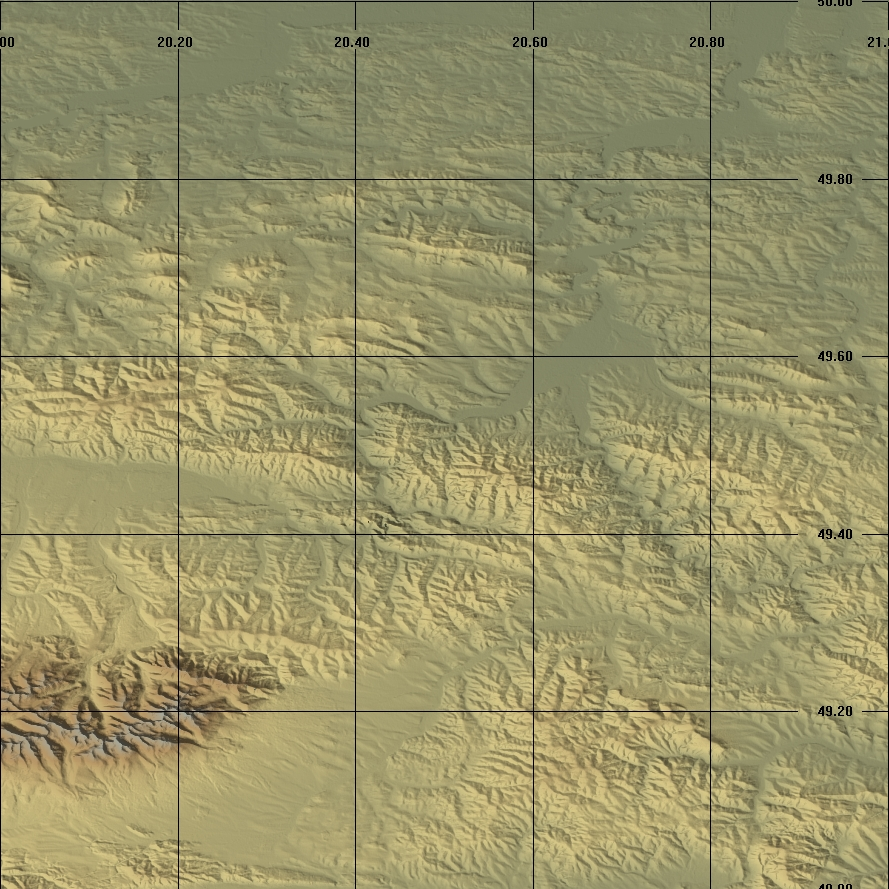
\includegraphics[width=0.6\linewidth]{img/srtm_example.jpg}
    \caption{Rzut pionowy danych SRTM 49-50N, 20-21E wygenerowany z wykorzystaniem oprogramowania 3DEM.}
    \label{fig:srtm-example}
\end{figure}

\par

Wykorzystując dane typu NMT możliwe jest wygenerowanie trójwymiarowej mapy terenu, a następnie rzutowanie jej na dwuwymiarową panoramę. Uzyskany w ten sposób obraz może zawierać dodatkowo informacje o szczytach górskich i może być dopasowany do wejściowego zdjęcia. Nakładając na siebie oba obrazy możemy zweryfikować widoczność poszczególnych szczytów - a dzięki temu następnie odrzucić te niewidoczne z~perspektywy użytkownika, a finalnie również etykietować te widoczne.


\par

Posiadając jedynie dane dotyczące geo-lokalizacji możliwe jest wygenerowanie modelu trójwymiarowego (cylindrycznego lub sferycznego) \cite{auto-terrain}\cite{peak-social-media}\cite{large-scale-visual} z danego punktu ziemi, a~następnie przeszukiwanie całej przestrzeni wokół obserwatora. Natomiast jeśli prócz lokalizacji dostępne są również informacje o polu widzenia urządzenia lub estymowana jest jego wartość możliwe jest przeprowadzenie dopasowania na płaskim obrazie. Ze względu na~mniejszą powierzchnię możliwych porównań podejście takie powinno dawać dokładniejsze wyniki. W przypadku opracowania Fedorov i in. \cite{peak-in-visual-content} obie opisane techniki są ze sobą łączone - przybliżane jest pole widzenia, które następnie rzutowane jest na przestrzeń trójwymiarową $\angle 360^{\circ}$.

\par

W pracy dyplomowej jednym z założeń było posiadanie danych  pochodzących z sensorów urządzenia, w~szczególności informacji dotyczących lokalizacji użytkownika, kątów obrotu urządzenia oraz specyfikacji technicznej zamontowanego w nim aparatu. Z tego powodu mogły być one wykorzystane przez badane algorytmy oraz poszczególne elementy opracowywanego projektu weryfikującego działanie procesu identyfikacji szczytów górskich na obrazie w czasie rzeczywistym. Takie dane pozwalają uzyskać dokładniejsze odwzorowanie terenu oraz generować panoramę terenu w taki sposób, jakby była widoczna z punktu, w~którym znajduje się obserwator oraz z takim samym polem widzenia. Może mieć to realny wpływ na skuteczność dopasowania obrazów oraz zmniejszyć złożoność algorytmów ze względu na ograniczenie przestrzeni, którą trzeba porównać ze zdjęciem wejściowym. 

\subsection{Bazy danych szczytów górskich} \label{section:geonames}

Projekt oraz platforma testowa tworzona w ramach pracy dyplomowej zasilana jest bazą danych nazw geograficznych \textit{GeoNames} \cite{geonames}. Jest to zbiór danych udostępnianych na licencji Creative Commons (CC) \cite{cc}. Kolekcja ta składa się z około $25$ milionów wpisów, z których prawie $60$ tysięcy dotyczy Polski. Baza danych podzielona została na różne kategorie takie jak wody, parki, miasta czy góry. Jednak, ze~względu na charakter pracy dyplomowej interesujące są jedynie wpisy dotyczące danych należących do ostatniego z~wymienionych typów. W Polsce zdefiniowano około $1200$ nazw gór, które stanowią kluczowe źródło informacji dla projektu podczas określania widocznych na wygenerowanym modelu szczytów. 

\par

Dane GeoNames podzielone są ze względu na kraj. System opracowany na potrzeby projektu pracy dyplomowej pobiera wpisy dla określonej puli krajów, następnie przetwarza je usuwając nieinteresujące typy oraz dane. W kolejnym kroku dzieli je ze względu na pola zależne od długości i szerokości geograficznej. Działania te pozwalają na zebranie dużej ilości danych na temat gór w wybranej przestrzeni geograficznej, co może przekładać się na precyzyjniejsze określanie widocznych szczytów. Podział na mniejsze zbiory pozwala zaoszczędzić pamięć operacyjną oraz moc obliczeniową potrzebną do~ewentualnego procesu filtrowania poszczególnych wpisów. 


\subsection{Rezultat przeglądu literatury - teoretyczne kroki procesu} \label{section:teoretical_pipeline}


Na podstawie przeprowadzonego przeglądu literatury stworzony został teoretyczny opis procesu rozpoznawania szczytów górskich. Na początku zakłada on wygenerowanie trójwymiarowego modelu topograficznego wykorzystując dane numeryczne SRTM. Na~takiej wizualizacji terenu określane mają być widoczne szczyty z bazy danych GeoNames. W trakcie kolejnego etapu użyte mają być algorytmy rozpoznawania konturów celem stworzenia obrazów binarnych z krawędziami gór na podstawie zwizualizowanej panoramy oraz zdjęcia rzeczywistego. Wygenerowane w ten sposób obrazy powinny być ze sobą porównane by określić podobieństwa poszczególnych ich wycinków w zależności od~badanego szczytu. Na podstawie takich wskaźników stwierdzona może być widoczność gór na~zdjęciu rzeczywistym. Wizualizację takiego hipotetycznego procesu w postaci diagramu przedstawiono na rysunku \ref{fig:teoretical-pipeline}. W dalszej części pracy w sposób bardziej szczegółowy przeanalizowano i opisano poszczególne elementy tego cyklu.

\begin{figure}[!h]
    \centering 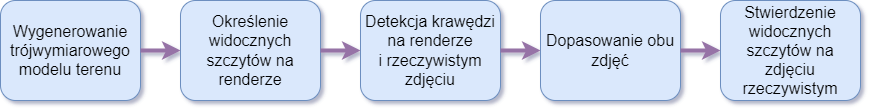
\includegraphics[width=1.0\linewidth]{img/flowchart_abstrakcja.drawio.png}
    \caption{Teoretyczne etapy procesu identyfikacji szczytów górskich na obrazie.}
    \label{fig:teoretical-pipeline}
\end{figure}

